\section{Versuchsdurchführung}
Der Versuch wurde entsprechend der Anweisungen aus der Laboranleitung \cite{Laboranleitung} durchgeführt.
Zu Beginn wurde unter Anleitung und Erklärung der Laborleitung Fr. Kupzok die
Funktionalität der Anlage geprüft und sichergestellt, dass Alles korrekt angeschlossen ist.\\
Die erste Messung hatte nun das Ziel den Generatorwirkungsgrad beider PV-Generatoren im Aufbau 2, also im DC-Betrieb zu bestimmen
und zusätzlich jeweils eine PV-Kennlinie aufzuzeichnen. Hierfür wurde die benötigte Messtechnik angeschlossen und ein verstellbarer Widerstand verschaltet.
Ebenfalls wurde die Bestrahlungsstärke mit einem Pyranometer gemessen.\\
\begin{figure}[!ht]
		\centering
		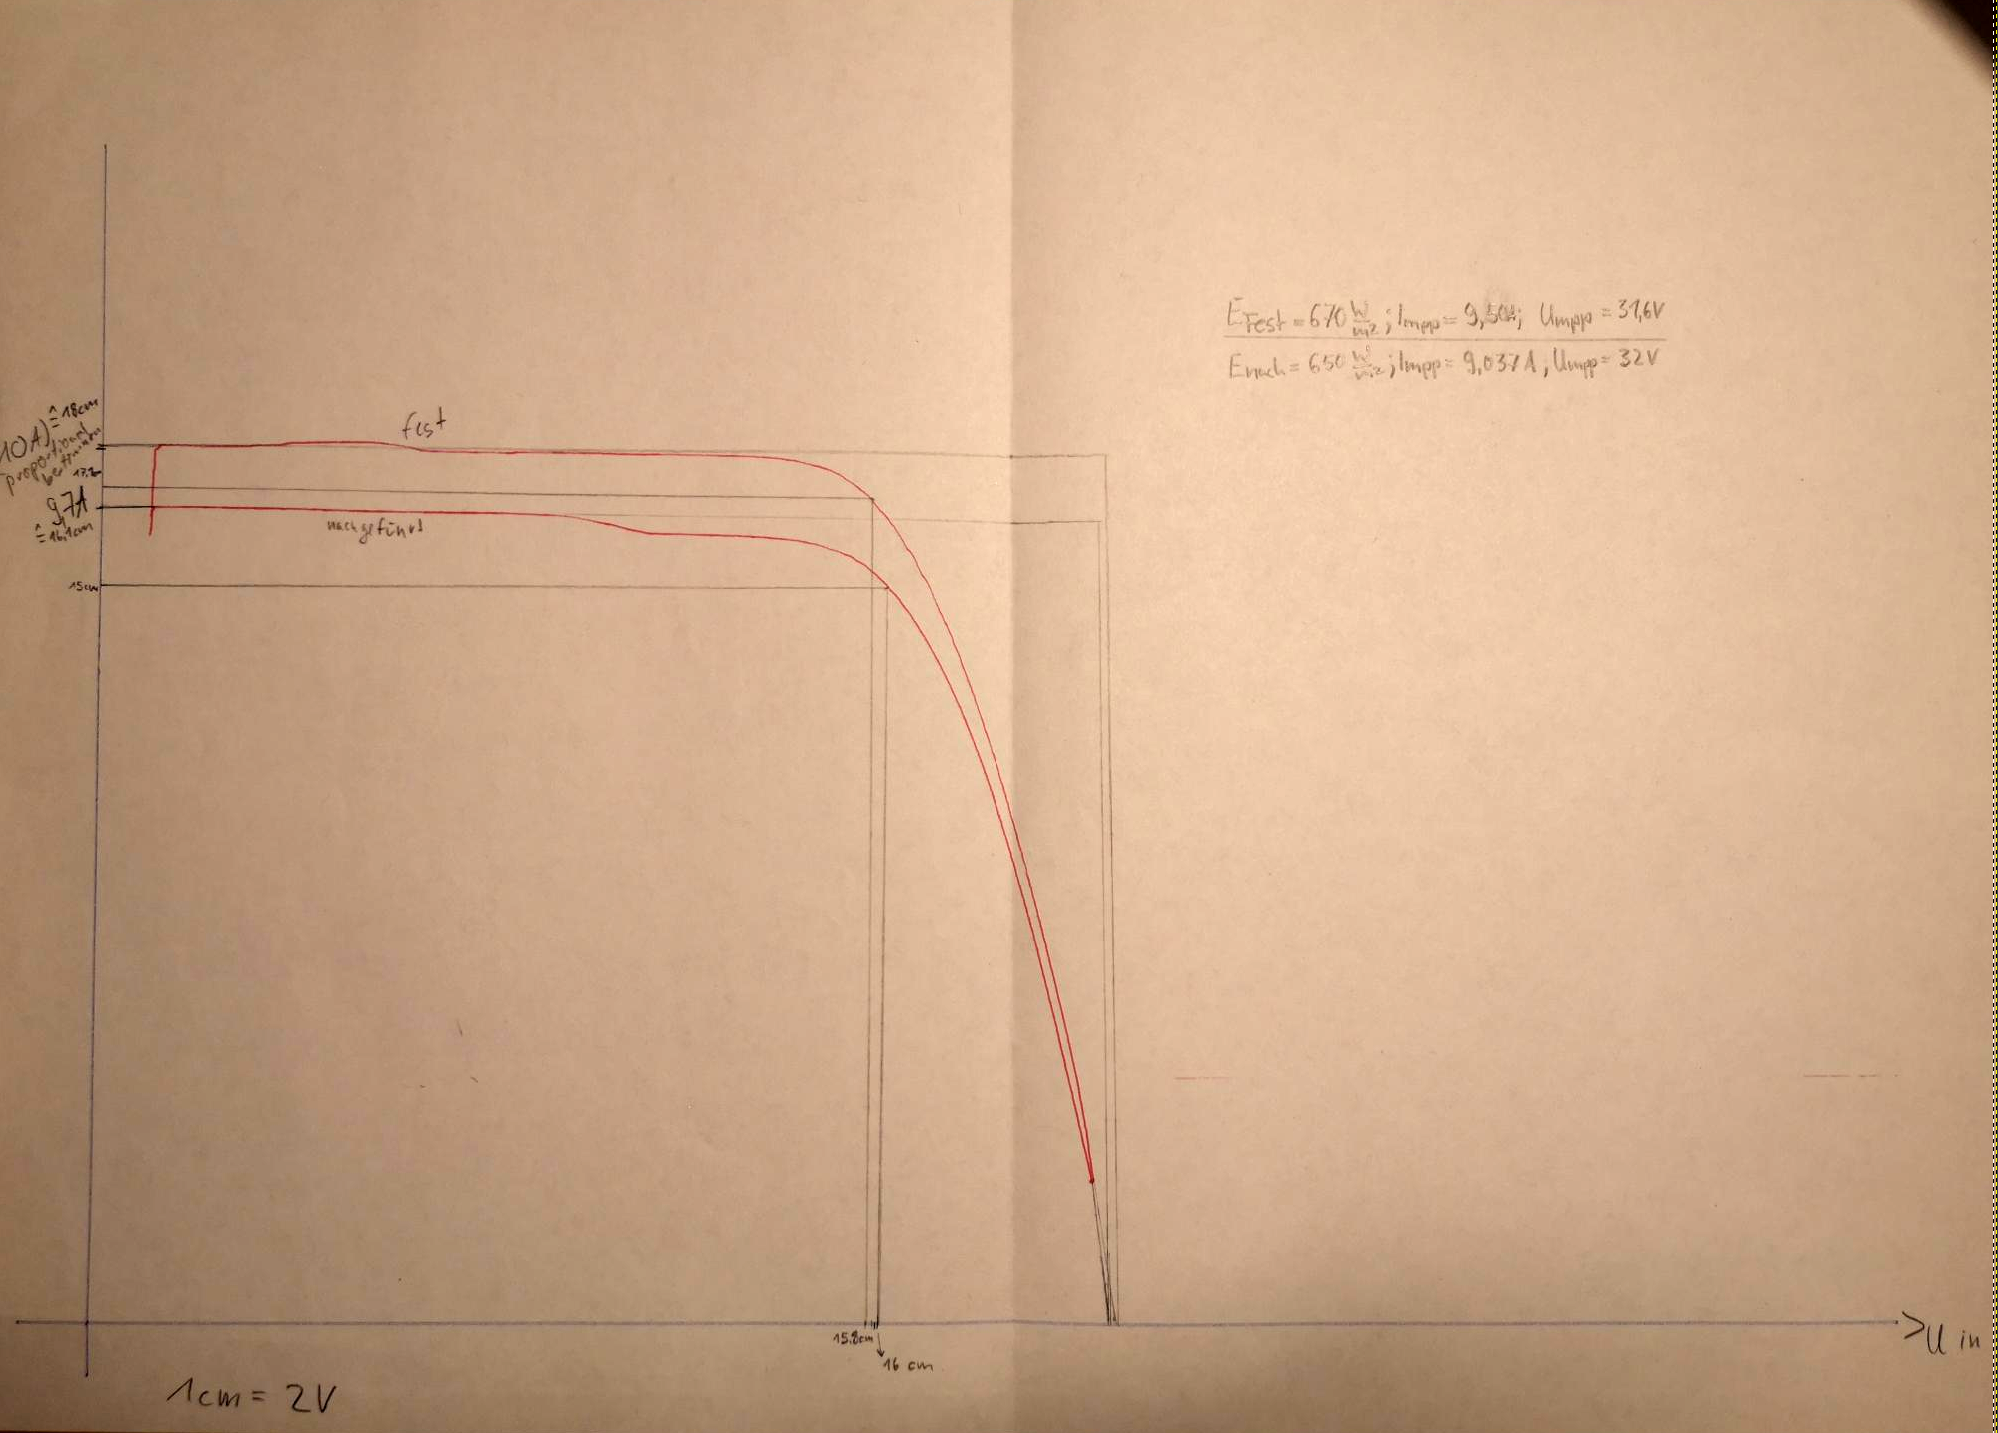
\includegraphics[width=0.7\textwidth]{Abbildungen/Kennlinie_PVGEN}
		\caption{Wirkungsgradkennlinie des PV-Generators in Abhängigkeit von der Bestrahlungsstärke}
		\label{fig:230514_PVGEN_Kennlinie}
\end{figure}

Mittels des verstellbaren Widerstandes wurde das System in den Leerlauf geführt und dann die Leerlaufspannung bestimmt.
Durch das Überbrücken des Widerstandes wurde dann ebenfalls der Kurzschlussfall herbeigeführt und der Kurzschlusstrom gemessen.\\
Im zweiten Teil des Versuches wurde nun Aufbau 1 verwendet, welcher den AC-Betrieb ermöglicht.
Ziel des zweiten Teils ist die Ermittlung der in der Anleitung \cite[S.8]{Laboranleitung} aufgeführten Kennwerte.\\
Hierzu gehören die Umgebungstemperatur, Bestrahlungsstärke, sowie Spannungen und Ströme an den relevanten Komponenten.
Zusätzlich wurde auch der zeitliche Spannungsverlauf des Wechselrichters auf der AC-Seite mit einem Oszillogramm aufgenommen.
Diese Kennwerte wurden für die folgenden Belastungsfälle bestimmt:
\begin{itemize}
    \item Ohne Last, nur der Wechselrichter ist in Betrieb
    \item geringe Ohmsche-induktive Last, Staubsauger Stufe 1
    \item mittlere Ohmsche-induktive Last, Staubsauger Stufe 2
    \item hohe Ohmsche-induktive Last, Staubsauger Stufe 3
    \item rein Ohmsche Last, S-Bahn-Heizung
\end{itemize}